\documentclass[11pt]{article}

\usepackage[margin=1in]{geometry}
\usepackage[T1]{fontenc}
\usepackage{lmodern}
\usepackage{microtype}
\usepackage{amsmath,amssymb,amsthm,mathtools}
\usepackage{mathrsfs}
\usepackage[dvipsnames]{xcolor}
\usepackage[most]{tcolorbox}
\usepackage{tikz}
\usepackage{enumitem}
\usepackage{tocloft}
\usepackage[hidelinks]{hyperref}

\definecolor{courseblue}{HTML}{1F4E79}
\definecolor{lightblue}{HTML}{EAF2F8}
\definecolor{lightgreen}{HTML}{EAF7EA}
\definecolor{lightpink}{HTML}{FCE8EF}
\definecolor{lightyellow}{HTML}{FFF8D6}
\definecolor{warningyellow}{HTML}{D6A000}
\definecolor{exercisebg}{HTML}{D6E6F5}
\definecolor{exerciseframe}{HTML}{1F4E79}
\definecolor{examplebg}{HTML}{F4FAFE}
\definecolor{exampleframe}{HTML}{85C1E9}
\definecolor{darkgray}{HTML}{333333}
\definecolor{lightorange}{HTML}{FDEBD8}
\definecolor{orangeframe}{HTML}{E08A3C}

\setlength{\parindent}{0pt}
\setlength{\parskip}{0.65em}
\setlist[itemize]{topsep=0.25em,itemsep=0.15em}
\renewcommand{\cftsecleader}{\cftdotfill{\cftdotsep}}
\renewcommand{\cftsubsecleader}{\cftdotfill{\cftdotsep}}

\theoremstyle{plain}
\newtheorem{theorem}{Theorem}[section]
\newtheorem{proposition}[theorem]{Proposition}
\newtheorem{lemma}[theorem]{Lemma}
\newtheorem{corollary}[theorem]{Corollary}
\theoremstyle{definition}
\newtheorem{definition}[theorem]{Definition}
\newtheorem{example}[theorem]{Example}
\newtheorem{exercise}[theorem]{Exercise}
\theoremstyle{remark}
\newtheorem*{remark}{Remark}
\newtheorem*{fact}{Fact}
\newtheorem*{warning}{Warning}

\tcolorboxenvironment{definition}{
  enhanced,
  unbreakable,
  colback=lightgreen,
  colframe=ForestGreen,
  boxrule=0.7pt,
  arc=2pt,
  left=6pt,
  right=6pt,
  top=5pt,
  bottom=5pt
}

\tcolorboxenvironment{warning}{
  enhanced,
  colback=lightyellow,
  colframe=warningyellow,
  boxrule=0.7pt,
  arc=2pt,
  left=6pt,
  right=6pt,
  top=5pt,
  bottom=5pt
}

\tcolorboxenvironment{exercise}{
  enhanced,
  colback=exercisebg,
  colframe=exerciseframe,
  boxrule=1pt,
  arc=2pt,
  left=6pt,
  right=6pt,
  top=5pt,
  bottom=5pt
}

\tcolorboxenvironment{example}{
  enhanced,
  colback=examplebg,
  colframe=exampleframe,
  boxrule=0.7pt,
  arc=2pt,
  left=6pt,
  right=6pt,
  top=5pt,
  bottom=5pt
}

\numberwithin{equation}{section}

\newcommand{\be}{\begin{eqnarray}}
\newcommand{\ee}{\end{eqnarray}}
\newcommand{\C}{\mathbb{C}}
\newcommand{\R}{\mathbb{R}}
\newcommand{\N}{\mathbb{N}}

\DeclareMathOperator{\Hol}{\mathcal{H}\mathrm{ol}}
\DeclareMathOperator{\Real}{Re}
\DeclareMathOperator{\Imag}{Im}
\newcommand{\A}{\mathcal{A}}
\newcommand{\CT}{\C[[T]]}
\newcommand{\CLT}{\C((T))}
\tcbset{breakable}
\begin{document}

\begin{center}
  \colorbox{lightblue}{%
    \begin{minipage}{0.94\textwidth}
      \vspace{0.55em}
      \begin{tabular*}{\textwidth}{@{\extracolsep{\fill}}lr}
        {\color{courseblue}\bfseries\LARGE Lecture 10} &
        {\color{courseblue}\bfseries\LARGE MATH 411}\\[0.35em]
        \textbf{Fall 2026} & \textbf{Date: Sep 25, 2026}\\
        & \textbf{Instructor: Manish Patnaik}
      \end{tabular*}
      \vspace{0.45em}
    \end{minipage}}
\end{center}

\setcounter{tocdepth}{1}
\tableofcontents
\vspace{0.45em}

% Handwritten page 1.
\section{Analytic functions are holomorphic}
We begin by recalling the definition from last time.

\noindent
\begin{minipage}[c]{0.62\textwidth}
\begin{definition}[Analytic]
\label{def:analytic}
Let $U\subseteq\C$ be open. A function $f\colon U\to\C$ is
\emph{analytic} if for each $z_0\in U$ there is a power series
$\sum a_nT^n$ with positive radius of convergence such that
\be
 f(z)=\sum a_n(z-z_0)^n\qquad\text{for all $z$ near $z_0$}.
\ee
\end{definition}
\end{minipage}\hfill
\begin{minipage}[c]{0.34\textwidth}
\centering
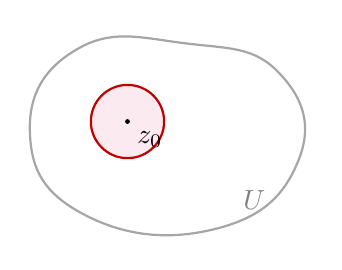
\begin{tikzpicture}[scale=0.62]
  \draw[thick,gray!70] plot[smooth cycle,tension=0.8]
    coordinates {(-2.6,0.2) (-1.6,1.9) (0.6,2.0) (2.5,1.4) (2.9,-0.4) (1.2,-1.8) (-1.5,-1.5)};
  \coordinate (z0) at (-0.6,0.4);
  \fill[lightpink,opacity=0.9] (z0) circle (0.75);
  \draw[red!75!black,thick] (z0) circle (0.75);
  \fill (z0) circle (1.4pt) node[below right]{$z_0$};
  \node[gray] at (2.0,-1.2) {$U$};
\end{tikzpicture}
\end{minipage}

\begin{remark}\leavevmode
\begin{enumerate}[label=(\arabic*)]
  \item We have not assumed anything else about $f$: no continuity, no
  differentiability. Everything below is a \emph{consequence} of having local
  power series expansions.
  \item If $\sum b_nT^n$ is a convergent power series on $D(0,r)$, then the
  function it defines on $D(0,r)$ is analytic (Lecture~9).
  \item If $\sum b_nT^n$ has radius of convergence $r>0$, then
  $f(z)=\sum b_nz^n$ is $\C$-differentiable at each $z\in D(0,r)$, and in fact
  \be
   f'(z)=\sum_{n\geq1}n\,b_nz^{n-1},\qquad\text{so}\qquad f'(0)=b_1.
  \ee
  That is, $f$ is holomorphic on $D(0,r)$ (Lecture~9).
\end{enumerate}
\end{remark}

% Handwritten page 2.
In fact $f'(z)$ is again given by a power series with radius of
convergence $r$, so it is also holomorphic by the same argument; and so are
$f''(z)$, $f'''(z)$, \dots. That is, $f$ is infinitely
$\C$-differentiable on $D(0,r)$. Moreover the coefficients can be read off
from the derivatives at $0$.

\begin{exercise}
Check that $f^{(k)}(0)=k!\,b_k$ for every $k\geq0$. \emph{Hint.} Writing
\be
 f(z)=b_0+b_1z+b_2z^2+\cdots,
\ee
we get $f(0)=b_0$, $f'(0)=b_1$, $f''(0)=2!\,b_2$, and in general only the
$n=k$ term of $f^{(k)}(z)=\sum_{n\geq k}n(n-1)\cdots(n-k+1)\,b_nz^{n-k}$
survives at $z=0$.
\end{exercise}

\begin{theorem}
\label{thm:analytic-hol}
Let $f$ be analytic on an open set $U$. Then $f$ is holomorphic on $U$ (in
fact infinitely $\C$-differentiable). Moreover, if at $z_0\in U$ we have an
expansion
\be
 f(z)=\sum b_n(z-z_0)^n\qquad\text{for $z$ near $z_0$},
\ee
then
\be
 b_k=\frac{f^{(k)}(z_0)}{k!}\qquad\text{for all }k\geq0.
 \label{eq:taylor-coeff}
\ee
\end{theorem}

\begin{proof}
Put $g(w)=\sum b_nw^n$, a convergent power series near $w=0$, so that
$f(z)=g(z-z_0)$ for $z$ near $z_0$. Translating the variable does not
affect difference quotients:
\be
 \frac{f(z+h)-f(z)}{h}=\frac{g\bigl((z-z_0)+h\bigr)-g(z-z_0)}{h}.
\ee
So near $z_0$, $f$ is infinitely $\C$-differentiable with
$f^{(k)}(z)=g^{(k)}(z-z_0)$, and by the exercise
$f^{(k)}(z_0)=g^{(k)}(0)=k!\,b_k$. Since $z_0\in U$ was arbitrary, the result
follows.
\end{proof}

In short:
\be
 f\ \text{analytic on }U\ \Longrightarrow\ f\ \text{holomorphic on }U.
\ee

\section{Functions vs series}

\newcommand{\hol}{\mathscr{H}}
\newcommand{\An}{\mathscr{A}}

For an open set $U\subseteq\C$, let us write
\be
 \An(U):=\{f\colon U\to\C\mid f\text{ is analytic on }U\} \text{ and also }
\ee
\be
 \hol(U):=\{f\colon U\to\C\mid
 f\text{ is holomorphic on }U,\text{ i.e., complex differentiable at every }z\in U\}.
\ee

Now we can equip $\hol(U)$ with the structure of a ring (actually a $\C$-algebra) in the natural way: if $f, g \in \hol(U)$, then $(f+g)(z):= f(z)+g(z)$ and and $(fg)(z):=f(z)g(z)$ are again holomorphic (so belong to $\hol(U)$) by what we saw earlier in class. We have just seen that $\An(U) \subset \hol(U)$ and we can ask the question : does this algebra structure preserve the space $\An(U)$? In other words, given $f, g$ analytic functions on $U$, is $f \cdot g$ and $f+g$ an analytic function on $U$? This is answered in the following lemma.

\begin{proposition} Let $f, g \in \An(U)$ be analytic functions on an open set $U$. Then $fg$ and $f+g$ are again analytic. \end{proposition}
\begin{proof} Let us just prove the first statement, as the second follows from a similar (and simpler) argument. Let $z_0 \in U$. As $f, g$ are analytic, there are power series $F(T)= \sum_{n} a_n T^n$ and $G(T) =\sum_n b_n T^n$ and an $s > 0$ so that $F, G$ both have radius of convergence $\geq s$ and such that $f(z) = F( z- z_0)$ and $g(z)=G(z-z_0)$ for $z \in D(z_0, s)$. What we need to argue is that there exists a power series $H(T):= \sum_{n}c_n T^n$ with radius of convergence $\geq s$ and such that $(f g)(z)= H(z - z_0)$ for $z \in D(z_0, s)$.  Set $c_n:=\sum_{k=0}^n a_k b_{n-k}.$ We claim that \be H(T)= F(T) G(T) = \sum_{n=0}^{\infty}c_nT^n \ee will work.  To establish this first observe:

\begin{lemma}
	\label{prop:prod-roc}
	Suppose $r>0$ and $f(T)=\sum a_nT^n$ and $g(T)=\sum b_nT^n$ both have radius
	of convergence at least $r$. Then
	\be
	f(T)\cdot g(T)=\sum c_nT^n,\qquad c_n=\sum_{k=0}^{n}a_kb_{n-k},
	\ee
	has radius of convergence $\geq r$.
\end{lemma}

\begin{warning}
Equality need not hold even when $F$ and $G$ both have radius $s$: for $s=1$, the series of $F(T)=(1+T)/(1-T)$ and $G(T)=(1-T)/(1+T)$ both have radius $1$, while $F(T)G(T)=1$ has infinite radius.
\end{warning}
\begin{proof}
	Since $f(T)$ and $g(T)$ have radius of convergence at least $r$, Hadamard's
	criterion gives
	\be
	\limsup_n|a_n|^{1/n}\leq\frac1r,\qquad\limsup_n|b_n|^{1/n}\leq\frac1r.
	\ee
	Pick any $0<s<r$.

	\emph{Claim.} There is a $C>0$ such that
	\be
	|a_n|\leq\frac C{s^n}\quad\text{and}\quad|b_n|\leq\frac C{s^n}
	\qquad\text{for all }n.
	\ee
	Indeed, since $0<s<r$ we have $\frac1s>\frac1r$, so there are only finitely
	many $n$ with $|a_n|^{1/n}\geq\frac1s$ (and likewise for $b_n$). For all
	other $n$ we have $|a_n|<s^{-n}$. Choosing $C\geq1$ larger than $|a_n|s^n$
	and $|b_n|s^n$ for these finitely many $n$, we get the desired bound.

	% Handwritten page 4.
	Now,
	\be
	|c_n|\leq\sum_{k=0}^{n}|a_k|\,|b_{n-k}|
	\leq\sum_{k=0}^{n}\frac C{s^k}\cdot\frac C{s^{n-k}}
	=\frac{C^2(n+1)}{s^n}.
	\ee
	Hence
	\be
	\limsup_n|c_n|^{1/n}\leq\limsup_n\frac{C^{2/n}(n+1)^{1/n}}{s}=\frac1s,
	\ee
	because $C^{2/n}\to1$ and $(n+1)^{1/n}=e^{\frac1n\log(n+1)}\to e^0=1$.
	Therefore the radius of convergence of $f g$ is $\geq s$. As $s<r$ was
	arbitrary, the radius of convergence of $f g$ is at least $r$.
\end{proof}





For every $|w|<s$, both $\sum_n|a_nw^n|$ and $\sum_n|b_nw^n|$ converge, so
\[
 \sum_{n=0}^{\infty}|c_nw^n|
 \leq \sum_{n=0}^{\infty}\sum_{k=0}^n
       |a_kw^k|\,|b_{n-k}w^{n-k}|
 =\left(\sum_{k=0}^{\infty}|a_kw^k|\right)
  \left(\sum_{j=0}^{\infty}|b_jw^j|\right)<\infty.
\]
Thus $H(T)=\sum_{n=0}^{\infty}c_nT^n$ has radius of convergence at least $s$.
The same absolute convergence lets us rearrange the double sum, giving
\[
 H(w)=\sum_{n=0}^{\infty}\sum_{k=0}^n a_kb_{n-k}w^n
 =\left(\sum_{k=0}^{\infty}a_kw^k\right)
  \left(\sum_{j=0}^{\infty}b_jw^j\right)=F(w)G(w).
\]
Taking $w=z-z_0$ shows that $(fg)(z)=H(z-z_0)$ on $D(z_0,s)$.
Since $z_0$ was arbitrary, $fg$ is analytic on $U$.



\end{proof}
\section{Uniqueness of power series expansions}
\emph{Question.} Suppose $f$ is analytic on $U\ni z_0$. Can we have two
different power series expansions $\sum a_nT^n$ and $\sum b_nT^n$ of $f$
near $z_0$?

\emph{Answer.} No! By \eqref{eq:taylor-coeff}, both $a_k$ and $b_k$ equal
$f^{(k)}(z_0)/k!$, a number determined by $f$ alone. The following
proposition gives a much stronger statement: a convergent power series is
already determined by its values on any set of points accumulating at the
centre.

% Handwritten page 3.
\begin{proposition}
\label{prop:identity}
\leavevmode
\begin{enumerate}[label=\textcircled{\scriptsize\arabic*}]
  \item \emph{(Isolated zeros.)} Let $f(T)\in\CT$ have positive radius of
  convergence $r$. Assume $f(T)\neq0$ (i.e.\ $f$ is not the power series
  $0+0\cdot T+0\cdot T^2+\cdots$), but $f(0)=0$. Then there exists $s>0$ such
  that
  \be
   f(z)\neq0\qquad\text{for all }z\in D(0,s),\ z\neq0.
  \ee
  \item \emph{(Identity principle.)} Let $f(T),g(T)\in\CT$ have positive
  radii of convergence, and suppose $f(z)=g(z)$ for all $z$ in an infinite
  subset of their common disc of convergence having $0$ as a point of
  accumulation. Then in fact $f(T)=g(T)$ as formal power series.
\end{enumerate}
\end{proposition}

\begin{center}
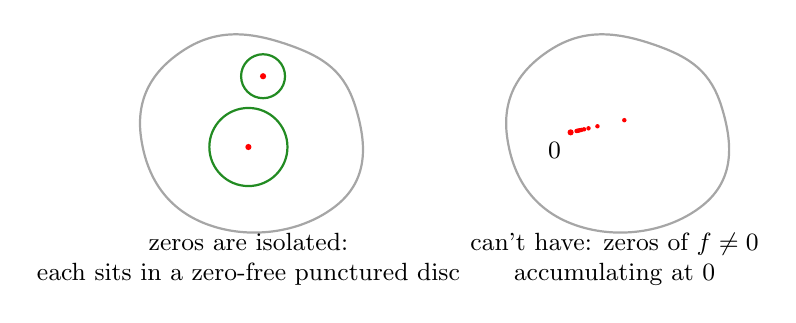
\begin{tikzpicture}[scale=0.62]
  % allowed picture
  \begin{scope}
    \draw[thick,gray!70] plot[smooth cycle,tension=0.8]
      coordinates {(-2.2,0) (-1.3,1.8) (0.8,1.9) (2.2,0.6) (1.8,-1.4) (-0.8,-1.8)};
    \draw[ForestGreen,thick] (0,-0.2) circle (0.8);
    \fill[red] (0,-0.2) circle (1.8pt);
    \draw[ForestGreen,thick] (0.3,1.25) circle (0.45);
    \fill[red] (0.3,1.25) circle (1.8pt);
    \node[font=\small,align=center] at (0,-2.5) {zeros are isolated:\\ each sits in a zero-free punctured disc};
  \end{scope}
  % forbidden picture
  \begin{scope}[xshift=7.5cm]
    \draw[thick,gray!70] plot[smooth cycle,tension=0.8]
      coordinates {(-2.2,0) (-1.3,1.8) (0.8,1.9) (2.2,0.6) (1.8,-1.4) (-0.8,-1.8)};
    \foreach \k in {1,...,9} {
      \fill[red] ({-0.9+1.1/\k},{0.1+0.25/\k}) circle (1.3pt);
    }
    \fill[red] (-0.9,0.1) circle (1.8pt) node[below left,black,font=\small]{$0$};
    \node[font=\small,align=center] at (0,-2.5) {can't have: zeros of $f\neq0$\\ accumulating at $0$};
  \end{scope}
\end{tikzpicture}
\end{center}

\begin{proof}
\textbf{\textcircled{\scriptsize1}$\Rightarrow$\textcircled{\scriptsize2}.}
Let $h(T)=f(T)-g(T)$. It is convergent wherever $f$ and $g$ are, so it has
positive radius of convergence, and $h(z)=f(z)-g(z)$ there. Now, as $h(z)$
is continuous, let $\{z_n\}$ be a sequence of distinct points of the given
subset, all nonzero, with $z_n\to0$ (possible since $0$ is a point of
accumulation). Then
\be
 f(z_n)=g(z_n)\ \Longrightarrow\ h(z_n)=0
 \ \Longrightarrow\ h(0)=\lim_{n\to\infty}h(z_n)=0.
\ee
% Handwritten page 4.
But if $h(T)\neq0$, then \textcircled{\scriptsize1} provides a punctured
disc $D(0,s)\setminus\{0\}$ on which $h$ has no zeros, whereas $z_n$ lies in
it for all large $n$. This contradicts the ``isolatedness'' of zeros. Hence
$h(T)=0$, i.e.\ $f(T)=g(T)$.

\textbf{Proof of \textcircled{\scriptsize1}.} Since $f(T)\neq0$, some
coefficient is nonzero; let $a_m$ be the first one. As $f(0)=a_0=0$, we have
$m\geq1$, and
\begin{align*}
 f(T)&=a_mT^m+\text{higher powers of }T\\
 &=a_mT^m\bigl(1+\underbrace{b_1T+b_2T^2+\cdots}_{h(T)}\bigr)
 =a_mT^m\bigl(1+h(T)\bigr),
 \qquad b_k:=\frac{a_{m+k}}{a_m}.
\end{align*}
Since $f(T)$ has positive radius of convergence, so does $h(T)$: it is
obtained from $f$ by dropping finitely many terms, shifting the powers, and
scaling, none of which changes the radius. Moreover, for $z\in D(0,r)$ we have
$f(z)=a_mz^m\bigl(1+h(z)\bigr)$ as functions.

Now $h(z)$ is continuous and $h(0)=0$. Choose a small neighbourhood
$D(0,s)$ of $0$, with $s\leq r$, such that $|h(z)|<1$ there. Then in this
neighbourhood,
\be
 f(z)=a_mz^m\bigl(1+h(z)\bigr),\qquad a_m\neq0,\quad 1+h(z)\neq0,
\ee
and this means that any zero of $f$ in this neighbourhood is at $z=0$.
\end{proof}

\begin{remark}
The integer $m\geq1$ in the proof is called the \emph{order} of the zero of
$f$ at $0$: near $0$, $f$ behaves like $a_mz^m$ times a function that does
not vanish.
\end{remark}

\end{document}
